\documentclass[11pt,a4paper]{article}
\usepackage[utf8]{inputenc}
\usepackage[T1]{fontenc}
\usepackage{ae}
\usepackage{mathtools}
\usepackage{amsfonts,amsmath,amssymb,amsthm}
\usepackage[libertine,cmintegrals,cmbraces,vvarbb]{newtxmath}
\usepackage[english]{babel}
\usepackage{cancel}
\usepackage{enumerate}
\usepackage[pdftex]{graphicx}
\usepackage{float}
\usepackage{caption}
\usepackage{subcaption}
\usepackage{listings}
\usepackage{fancyhdr}
\pagestyle{fancy}
\usepackage{fancybox}
\usepackage[dvipsnames]{xcolor}
\usepackage{tikz}
\usetikzlibrary{matrix,arrows,decorations.pathmorphing}
\usepackage{verbatim}
\usepackage{marvosym}
\usepackage{algorithm2e}
\usepackage{color}
\usepackage{bm}
\usepackage{todonotes}

\makeatletter
\newcommand\todoname{todo}
\newcommand\listtodoname{List of todos}
\makeatother

\setlength{\parindent}{0em}

\newcommand{\F}[0]{\mathbb{F}}
\newcommand{\N}[0]{\mathbb{N}}
\newcommand{\Z}[0]{\mathbb{Z}}
\newcommand{\Q}[0]{\mathbb{Q}}
\newcommand{\R}[0]{\mathbb{R}}
\newcommand{\C}[0]{\mathbb{C}}
\newcommand{\B}[0]{\mathbb{B}}
\newcommand{\im}[0]{\mathit{i}}
\newcommand{\uber}[2]{{{#1} \choose {#2}}}
\newcommand{\vect}[1]{\begin{pmatrix}#1\end{pmatrix}}
\newcommand{\norm}[1]{\left\lvert #1 \right\rvert}

\def\students{Willi Gierke, Arik Elimelech, Mehmed Halilovic, Leon Sixt}

\fancyhead[L]{SS 2017}
\fancyhead[C]{Maschinelles Lernen 2}
\fancyhead[R]{Assignment 02 -- \textbf{ESHG}}
\fancyfoot[L]{}
\fancyfoot[C]{\students}
\fancyfoot[R]{}


\title{Machine Learning 2 -- Group ESHG \\
        Assignment 02
}

\author{\students}
\date{\today}

\begin{document}
\maketitle

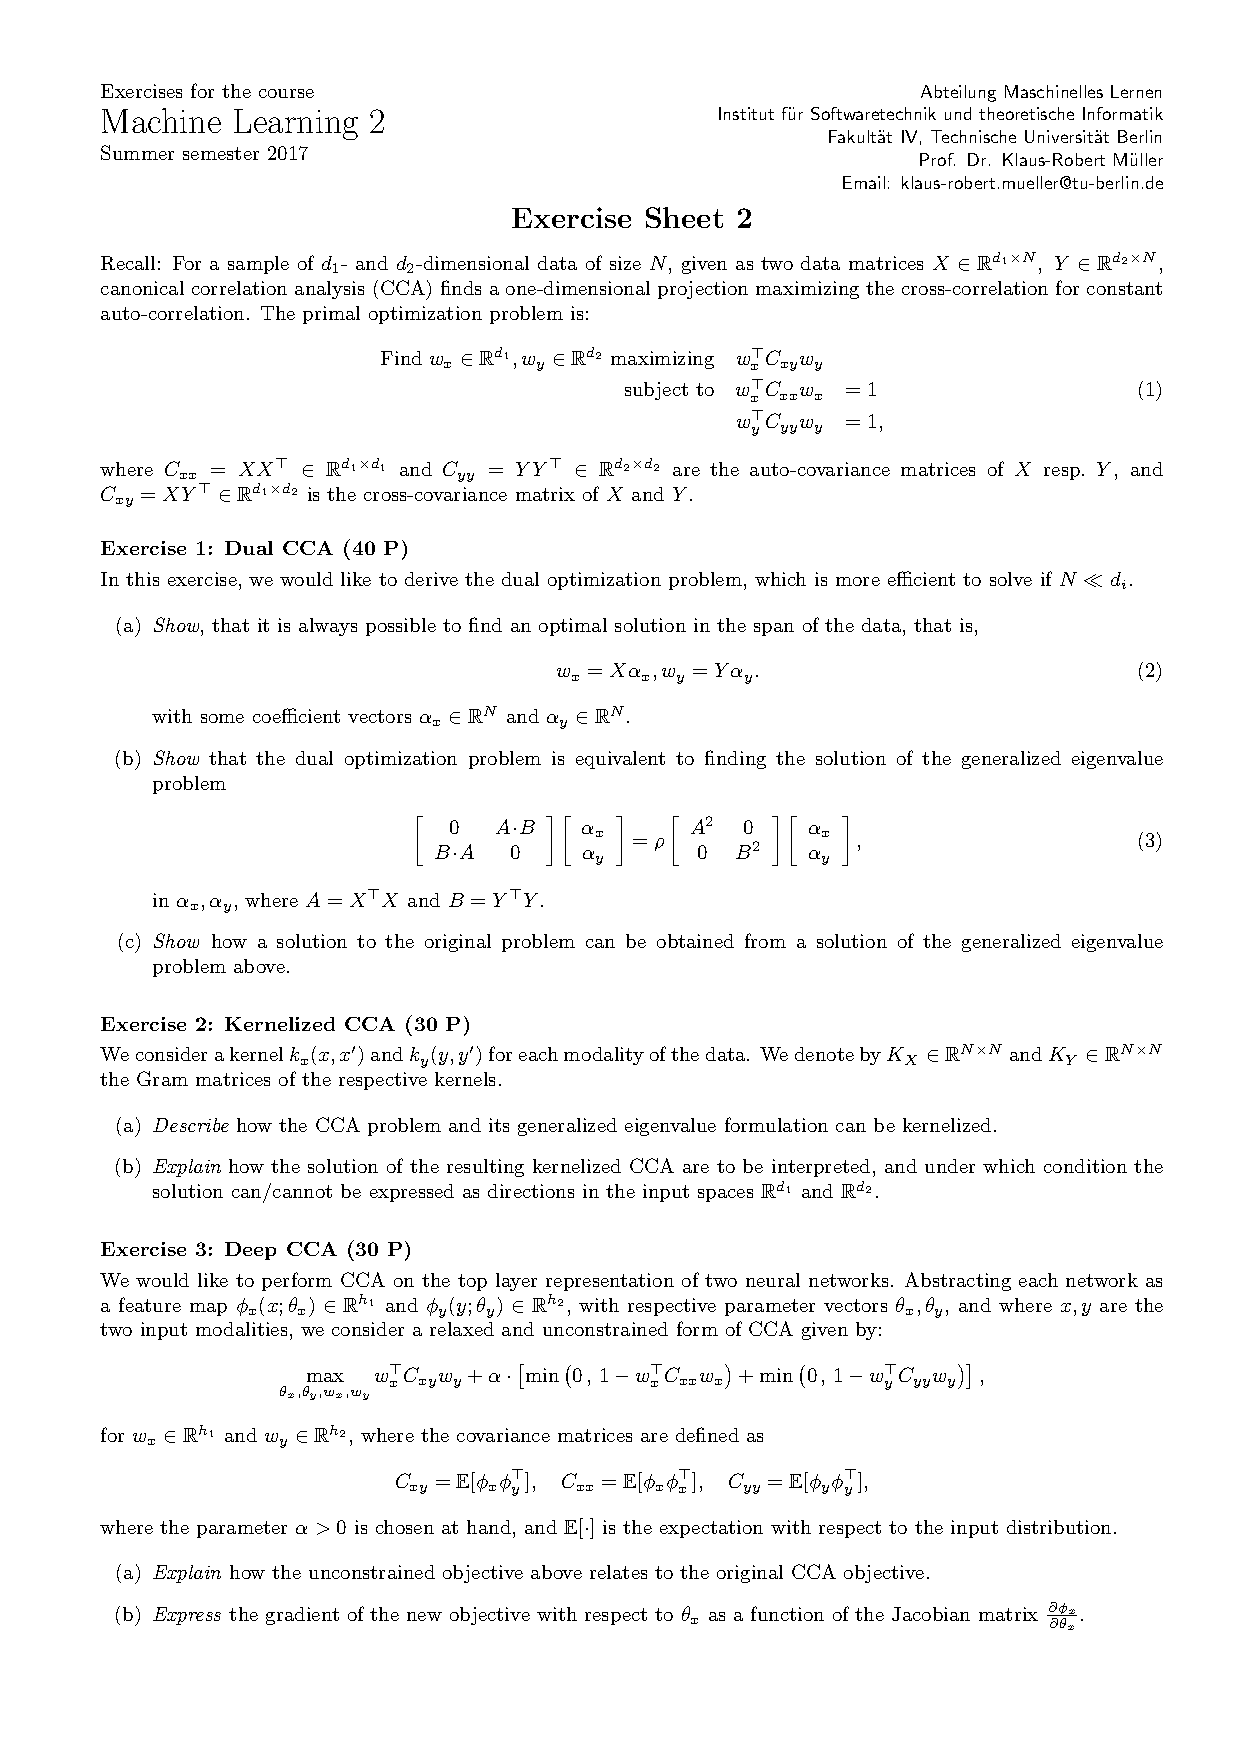
\includegraphics[clip, trim=0.5cm 5cm 0.5cm 3cm, width=1.00\textwidth]{sheet02.pdf}

\clearpage

\section*{Task 1}

\subsection*{a}
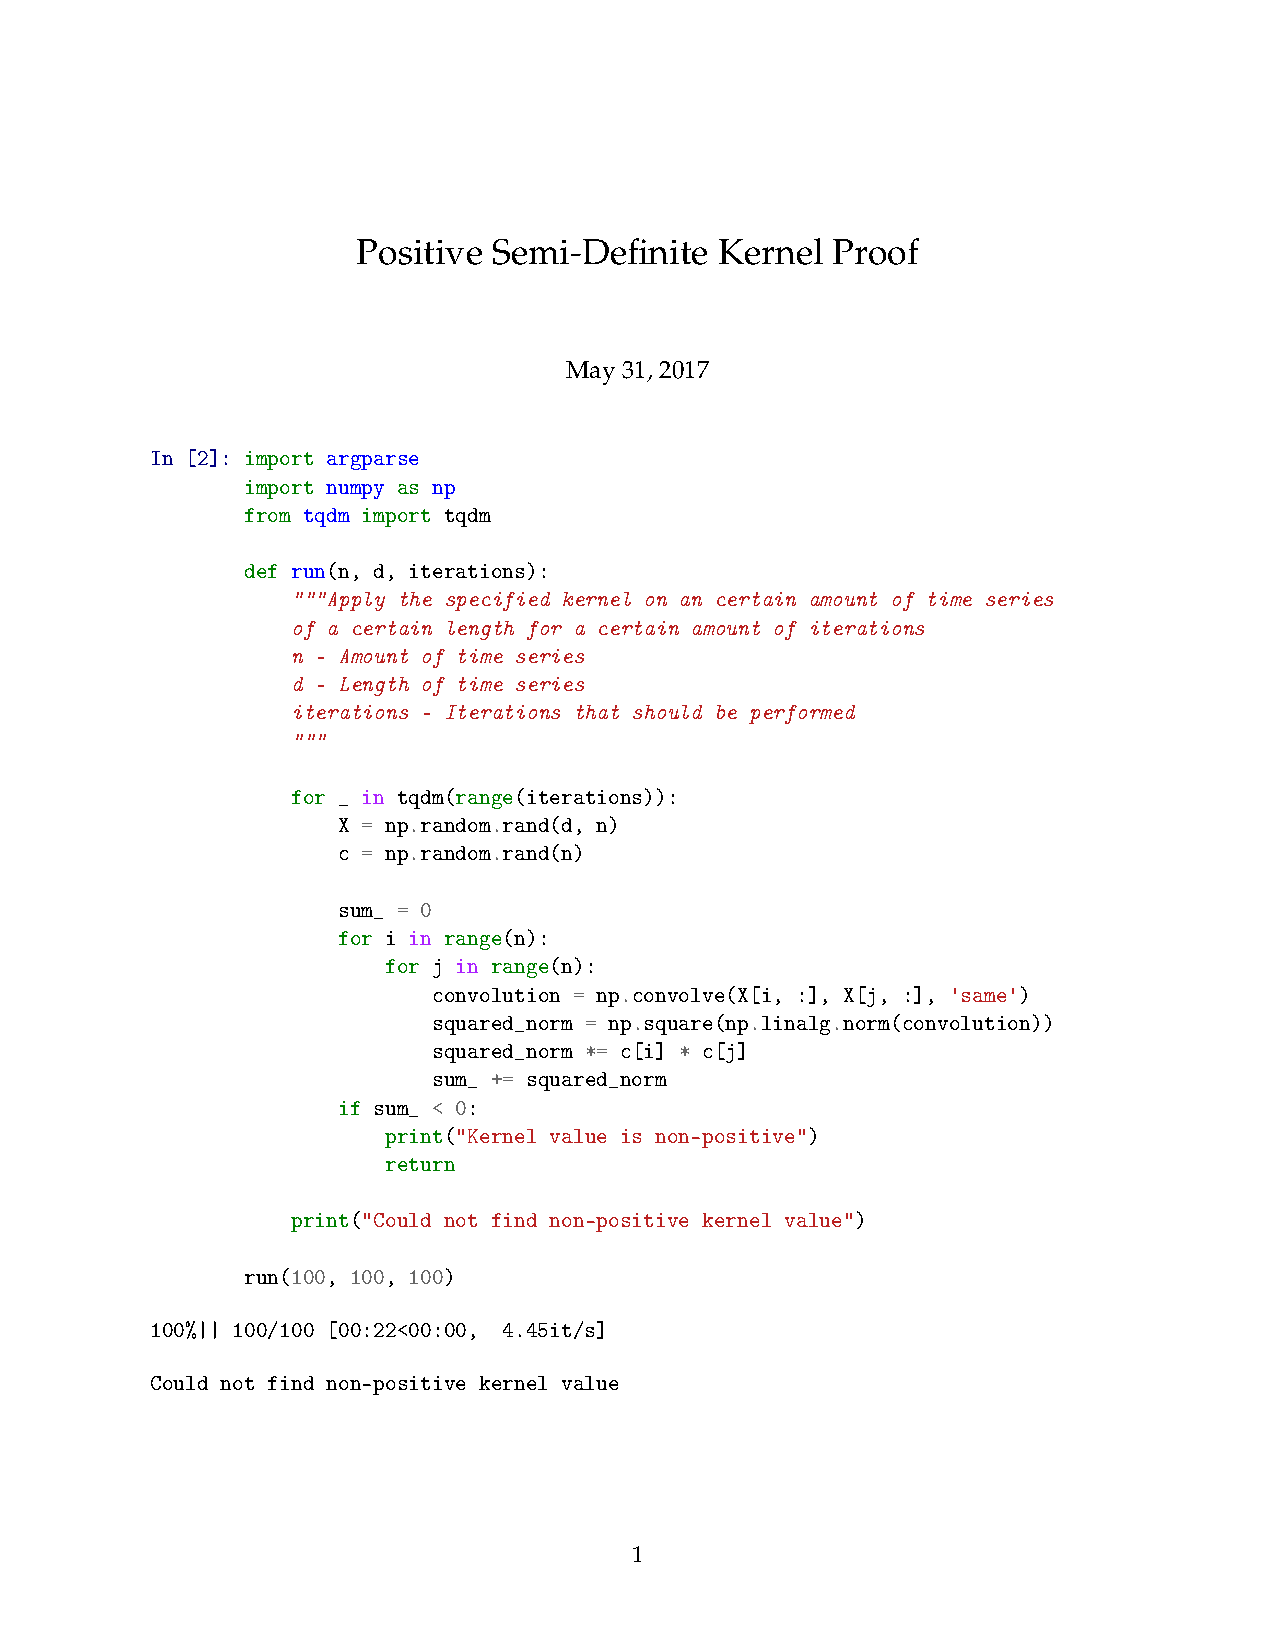
\includegraphics[clip, trim=0.5cm 2.5cm 0.5cm 4cm, width=0.90\textwidth]{KernelProof.pdf}

\subsection*{b}

The kernel is given by:

\begin{equation}
    k(x, y) = \lVert x * y \rVert ^ 2
\end{equation}

To be positive semi-definite, the kernel has to fulfill:

\begin{equation}
    \sum_{i=1}^n \sum_{j=1}^n c_i c_j k(x_i, x_j)
\end{equation}
for $n \in \N$, $\{x_1, \ldots, x_n\} \in \R^{d \times n} $ and $c \in \R^n$.
\\
\\
For the given kernel:
\begin{align}
    \sum_{i=1}^n \sum_{j=1}^n c_i c_j \lVert x_i * x_j \rVert ^ 2  \\
    = \sum_{i=1}^n \sum_{j=1}^n c_i c_j \sum_{t=0}^T (x_i * x_j)_t^2  \\
\end{align}

We can rewrite the convolution as fourier transformation.
Here, $\hat x_i $ denotes the fourier transform of $x_i$ and $F^{-1}$ the inverse
fourier transformation.
\begin{align}
    & \lVert x_i * x_j \rVert ^ 2 = \\
    &    = \Vert F^{-1}(\hat x_i \cdot  \hat x_j) \rVert ^ 2  \\
\end{align}

We assume that the feature space, ask for in the exercise, is connected to the
fourier transformation of x. However, the inverse fourier transform obstruct
us to separate the kernel into two feature maps.

\section*{Task 2}


\section*{Task 3}
\subsection*{i}

\begin{gather*}
C = \sum_j p_j \log(\frac{p_j}{q_j}) \\
\frac{\partial C}{\partial q_i} = p_i * \frac{\partial}{\partial q_i} \log(\frac{p_i}{q_i}) \\
\frac{\partial C}{\partial q_i} = p_i * \frac{q_i}{p_i} * (-\frac{p_i}{q_i^2}) \\
\frac{\partial C}{\partial q_i} = -\frac{p_i}{q_i} \\
\end{gather*}

\subsection*{ii}
\begin{gather*}
\frac{\partial C}{\partial x_i} = \frac{\partial C}{\partial \vec{q}} \frac{\partial \vec{q}}{\partial x_i} \\
\text{As we just have shown}\\
(\frac{\partial C}{\partial \vec{q}})_j = \frac{\partial C}{\partial q_j} = -\frac{p_j}{q_j} \quad .\\
\text{For the second factor we get} \\
(\frac{\partial \vec{q}}{\partial x_i})_j = \frac{\partial q_j}{\partial x_i} = \frac{\partial}{\partial x_i} \frac{e^{x_j}}{\sum_k e^{x_k}} \\
= \frac{e^{x_j} \sum_k e^{x_k} \delta_{ij} - e^x_i e^x_j}{\big[ \sum_k e^{x_k} \big]^2} \\
= \frac{e^{x_j} \delta_{ij}}{\sum_k e^{x_k}} - \frac{e^{x_i}}{\sum_k e^{x_k}} \frac{e^{x_j}}{\sum_k e^{x_k}} \\
= q_j \delta_{ij} - q_i q_j \\
\xRightarrow[]{}
\frac{\partial C}{\partial \vec{q}} \frac{\partial \vec{q}}{\partial x_i} = \sum_j (-\frac{p_j}{q_j})(q_j \delta_{ij} - q_iq_j) \\
= \sum_j (-\frac{p_j q_j \delta_{ij}}{q_j})+(\frac{p_j q_iq_j}{q_j}) \\
= \sum_j (-p_j \delta_{ij})+(p_j q_i)\\
= \sum_j p_jq_i - \sum_j p_j \delta_{ij} \\
= q_i \sum_j p_j - p_i
= q_i - p_i
\end{gather*}

\subsection*{iii}
\textbf{Stability/Boundedness:} The first derivative has $q_i$ in the denominator which can become close to zero.
In that case the gradient would go to infinity.
The second derivative only consists of a sum which performs better in these aspects. \\
\textbf{Validity:} To perform a gradient descent we can only vary the projected points $x_i$ so it's more meaningful to calculate the derivative with respect to $x_i$.

\todo[inline]{Finish this task}

\clearpage


\end{document}
